\begin{figure}[t]
    \definecolor{YellowGreen}{RGB}{49,126,53}
    \definecolor{Rhodamine}{RGB}{243,156,146}
    \definecolor{Dandelion}{RGB}{242,193,106}
    \vspace{-0.5\baselineskip}
    \centering
    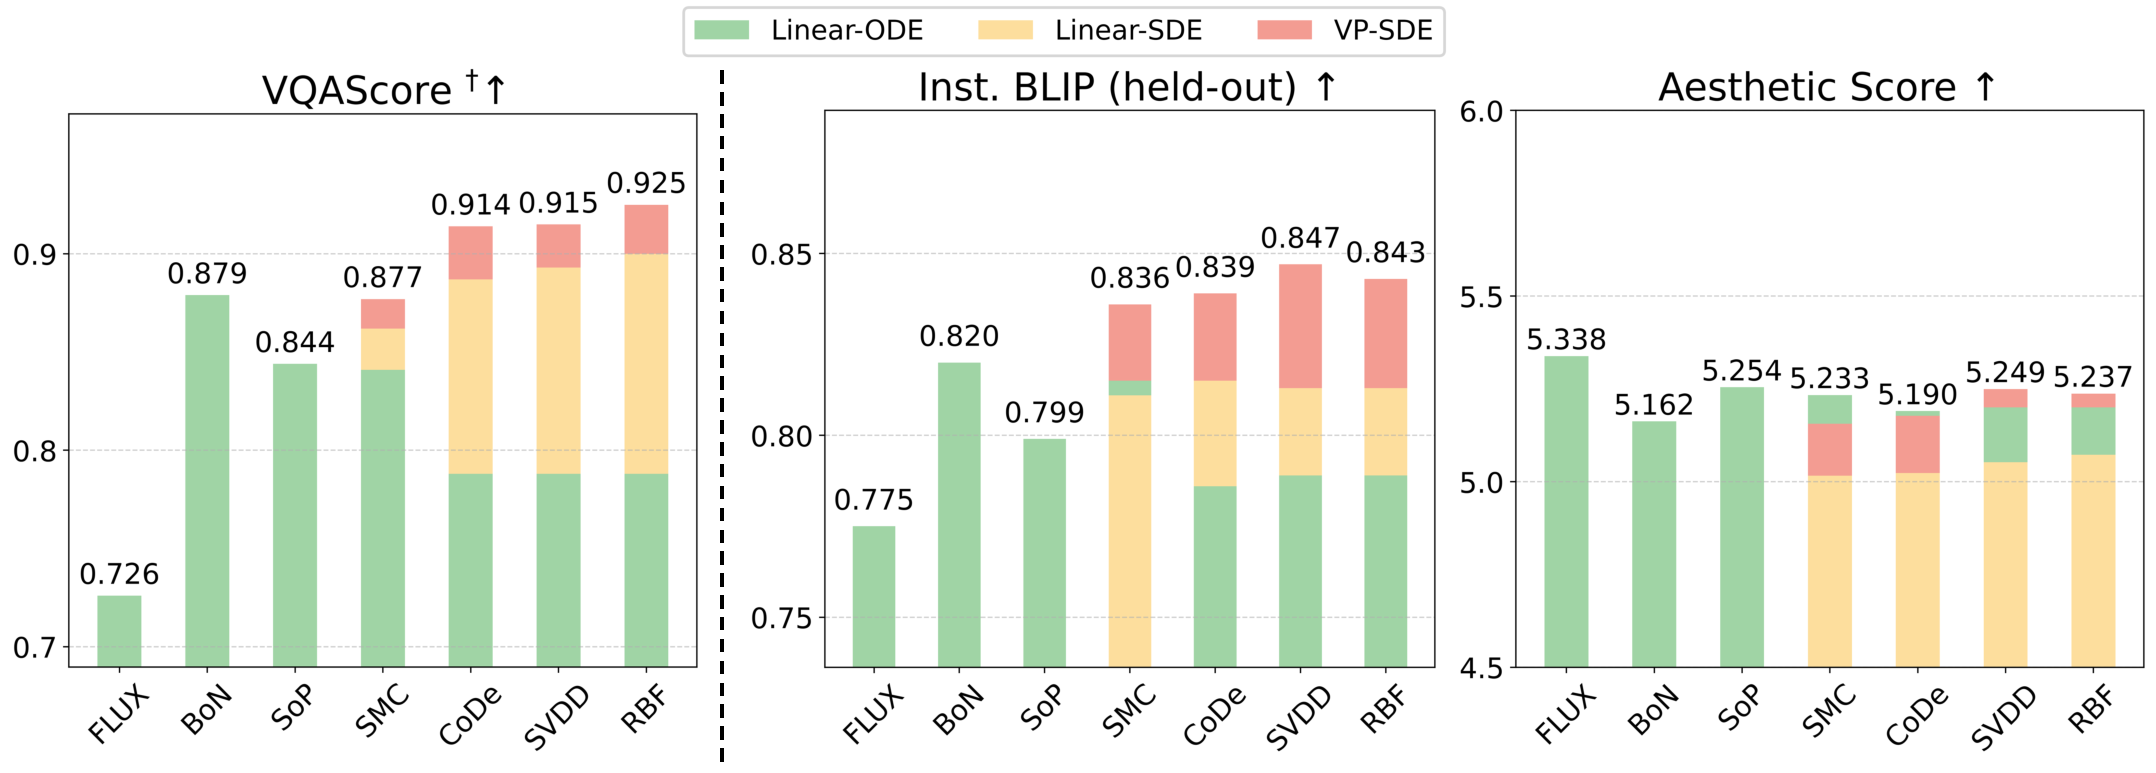
\includegraphics[width=1.0\linewidth]{Tables/compo_bar_graph/compo_bar_graph.pdf}
    \caption{\textbf{Quantitative results of compositional text-to-image generation.} \textsuperscript{\textdagger} denotes the given reward used in inference-time scaling (left). 
    Notably, performance consistently improves from {\color{YellowGreen}Linear-ODE} to {\color{Dandelion}Linear-SDE} and {\color{Rhodamine}VP-SDE} for both given and held-out rewards (left, middle), without significant quality degradation, as evidenced by the comparable aesthetic score~\cite{Schuhmann:aesthetics} (right).} 
    \label{fig:composition_main}
    \vspace{-0.75\baselineskip}
\end{figure}

% \begin{table*}[!t]
% \setlength{\tabcolsep}{1.5pt}
% \centering
% \scriptsize
% \renewcommand{\arraystretch}{1.2} 
% \caption{\textbf{Quantitative results of compositional image generation.} \textsuperscript{\textdagger} denotes the given reward used in inference-time scaling. The best result in the given and held-out reward is highlighted by \textbf{bold}, and the runner-up is \underline{underlined}. L.O., L.S., and V.S. indicate Linear-ODE, Linear-SDE, and VP-SDE.}
% \vspace{-0.5\baselineskip}
% \label{tab:composition_main}
% \newcolumntype{X}{>{\centering\arraybackslash}m{0.13\linewidth}}
% \newcolumntype{Y}{>{\centering\arraybackslash}m{0.065\linewidth}}
% \newcolumntype{W}{>{\centering\arraybackslash}m{0.045\linewidth}}
% \begin{tabular}{X | Y Y Y | W W W | W W W | W W W | W W W }
% \toprule
% \multirow{2}{*}{Metric} & 
% \multirow{1}{*}{\makecell{FLUX~\cite{BlackForestLabs:2024Flux}}} & 
% \multirow{1}{*}{BoN} & 
% \multirow{1}{*}{\makecell{SoP~\cite{Ma2025:SoP}}} & 
% \multicolumn{3}{c|}{SMC~\cite{Kim:2025DAS}} & 
% \multicolumn{3}{c|}{CoDe~\cite{Singh:2025CoDE}} & 
% \multicolumn{3}{c|}{SVDD~\cite{Li2024:SVDD}} & 
% \multicolumn{3}{c}{{\Oursbf{}} (Ours)} \\
% \cline{2-16}
% & \multicolumn{3}{c|}{L.O.} & L.O. & L.S. & V.S. & L.O. & L.S. & V.S. & L.O. & L.S. & V.S. & L.O. & L.S. & V.S. \\
% \hline
% \makecell{VQAScore\textsuperscript{\textdagger}\\\cite{Lin:2024CLIPFlanT5}~$\uparrow$} & 
% 0.726 & 0.879 & 0.844 & 
% 0.841 & 0.862 & 0.877 & 
% 0.788 & 0.887 & 0.914 & 
% 0.788 & 0.893 & \underline{0.915} & 
% 0.788 & 0.900 & \textbf{0.925} \\
% \hline
% Inst. BLIP~\cite{Dai:2023InstructBLIP}~$\uparrow$ (held-out) & 
% 0.775 & 0.820 & 0.799 & 
% 0.815 & 0.811 & 0.836 & 
% 0.786 & 0.815 & 0.839 & 
% 0.789 & 0.813 & \textbf{0.847} & 
% 0.789 & 0.813 & \underline{0.843} \\
% \hline
% Aesthetic Score~\cite{Schuhmann:aesthetics}~$\uparrow$ & 
% 5.338 & 5.162 & 5.254 & 
% 5.233 & 5.016 & 5.156 & 
% 5.190 & 5.023 & 5.177 & 
% 5.200 & 5.052 & 5.249 & 
% 5.200 & 5.072 & 5.237 \\
% \bottomrule
% \end{tabular}
% \vspace{-0.75\baselineskip}
% \end{table*}




% =============================================================================== %
% Multicolumn Multirow error in cline.
% \begin{table*}[!t]
%     \setlength{\tabcolsep}{1.5pt}
%     \centering
%     \scriptsize
%     \newcommand{\good}[1]{\tiny{\textcolor{blue}{+#1\%}}}
%     \newcommand{\bad}[1]{\tiny{\textcolor{red}{-#1\%}}}
%     \caption{\textbf{Quantitative results of compositional image generation.} \textsuperscript{\textdagger} denotes the given reward used in inference-time scaling. For particle-based sampling methods, the relative improvement in each cell is computed with respect to the Linear-ODE case. The best result in the given and held-out reward is highlighted by \textbf{bold}, and the runner-up is \underline{underlined}. L.O., L.S., and V.S. indicate Linear-ODE, Linear-SDE, and VP-SDE, respectively. \textsuperscript{*} denotes results with $50$ denoising steps.}
%     \vspace{-0.5\baselineskip}
%     \label{tab:composition_main}
%     \newcolumntype{X}{>{\centering\arraybackslash}m{0.12\linewidth}}
%     \newcolumntype{Y}{>{\centering\arraybackslash}m{0.04\linewidth}}
%     \newcolumntype{W}{>{\centering\arraybackslash}m{0.06\linewidth}}
%     \begin{tabular}{X | W W W | W Y Y | W Y Y | W Y Y | W Y Y }
%         \toprule
%         \multirow{2}{*}{\makecell{Metric}} & 
%         \multirow{2}{*}{FLUX} & \multirow{2}{*}{BoN} & \multirow{2}{*}{\makecell{SoP~\cite{Ma2025:SoP}}} & \multicolumn{3}{c|}{\multirow{2}{*}{SMC~\cite{Kim:2025DAS}}} & \multicolumn{3}{c|}{\multirow{2}{*}{CoDe~\cite{Singh:2025CoDE}}} & \multicolumn{3}{c|}{\multirow{2}{*}{SVDD~\cite{Li2024:SVDD}}} & \multicolumn{3}{c}{\multirow{2}{*}{{\Oursbf{}} (Ours)}} \\
%         \cline{2-16}
%         & \multicolumn{3}{c|}{L.O.} & L.O. & L.S. & V.S. & L.O. & L.S. & V.S. & L.O. & L.S. & V.S. & L.O. & L.S. & V.S. \\
%         \hline
%         \makecell{VQAScore\textsuperscript{\textdagger}\\\cite{Lin:2024CLIPFlanT5} $\uparrow$} & 0.726 & 0.879 & 0.844 & 0.841 & \makecell{0.862} & \makecell{0.877} & 0.788 & \makecell{0.887} & \makecell{0.914} & 0.788 & \makecell{0.893} & \makecell{\underline{0.915}} & 0.788 & \makecell{0.900} & \makecell{\textbf{0.925}} \\
%         \hline
%         \makecell{Inst. BLIP~\cite{Dai:2023InstructBLIP} $\uparrow$ \\ (held-out)} & 0.775 & 0.820 & 0.799 & 0.815 & \makecell{0.811} & \makecell{0.836} & 0.786 & \makecell{0.815} & \makecell{0.839} & 0.789 & \makecell{0.813} & \makecell{\textbf{0.847}} & 0.789 & \makecell{0.813} & \makecell{\underline{0.843}} \\
%         \hline
%         \makecell{Aesthetic \\ Score~\cite{Schuhmann:aesthetics} $\uparrow$} & 5.338 & 5.162 & 5.254 & 5.233 & 5.016 & 5.156 & 5.190 & 5.023 & 5.177 & 5.200 & 5.052 & 5.249 & 5.200 & 5.072 & 5.237 \\
%         \bottomrule
%     \end{tabular}
%     \vspace{-0.25\baselineskip}
% \end{table*}



% % =============================================================================== %
% % ===================== 3/8 16:47 Juil's Update ================================= %
% % =============================================================================== %
% \begin{table*}[!t]
%     \setlength{\tabcolsep}{1.5pt}
%     \centering
%     \scriptsize
%     \newcommand{\good}[1]{\tiny{\textcolor{blue}{+#1\%}}}
%     \newcommand{\bad}[1]{\tiny{\textcolor{red}{-#1\%}}}
%     \caption{\textbf{Quantitative results of compositional image generation.} \textsuperscript{\textdagger} denotes the given reward used in inference-time scaling. For particle-based sampling methods, the relative improvement in each cell is computed with respect to the Linear-ODE case. The best result in the given and held-out reward is highlighted by \textbf{bold}, and the runner-up is \underline{underlined}. L.O., L.S., and V.S. indicate Linear-ODE, Linear-SDE, and VP-SDE, respectively. \textsuperscript{*} denotes results with $50$ denoising steps.}
%     \vspace{-1.0\baselineskip}
%     \label{tab:composition_main}
%     \newcolumntype{X}{>{\centering\arraybackslash}m{0.095\linewidth}}
%     \newcolumntype{Y}{>{\centering\arraybackslash}m{0.045\linewidth}}
%     \newcolumntype{Z}{>{\centering\arraybackslash}m{0.05\linewidth}}
%     \newcolumntype{W}{>{\centering\arraybackslash}m{0.035\linewidth}}
%     \begin{tabular}{X | Y Y | Z Z | W W W | W Y Y | W Y Y | W Y Y | W Y Y }
%         \toprule
%         \multirow{4}{*}{\makecell{Metric}} & \multicolumn{4}{c|}{\textbf{Diffusion Model}} & \multicolumn{15}{c}{\textbf{Flow Model}} \\
%         \cline{2-20}
%         & \multirow{2}{*}{SD2} & \multirow{2}{*}{$\text{SD2}^{*}$} & \multicolumn{2}{c|}{SVDD~\cite{Li2024:SVDD}} & \multirow{2}{*}{FLUX} & \multirow{2}{*}{BoN} & \multirow{2}{*}{\makecell{SoP\\\cite{Ma2025:SoP}}} & \multicolumn{3}{c|}{\multirow{2}{*}{SMC~\cite{Kim:2025DAS}}} & \multicolumn{3}{c|}{\multirow{2}{*}{CoDe~\cite{Singh:2025CoDE}}} & \multicolumn{3}{c|}{\multirow{2}{*}{SVDD~\cite{Li2024:SVDD}}} & \multicolumn{3}{c}{\multirow{2}{*}{{\Oursbf{}} (Ours)}}\\
%         & & & SD2 & SD2$^{*}$ & & & & & & & & & & & & & & \\
%         % & \multirow{2}{*}{\makecell{SD}} & \multirow{2}{*}{\makecell{$\text{SD}^{*}$}} & \multicolumn{2}{c}{SVDD~\cite{Li2024:SVDD}} & \multirow{2}{*}{FLUX} & \multirow{2}{*}{BoN} & \multirow{2}{*}{SoP~\cite{Ma2025:SoP}} & \multirow{2}{*}{\multicolumn{3}{c|}}{\makecell{SMC \\ \cite{Kim:2025DAS}}} & \multirow{2}{*}{\multicolumn{3}{c|}{\makecell{CoDe \\ \cite{Singh:2025CoDE}}}} & \multirow{2}{*}{\multicolumn{3}{c|}{\makecell{SVDD\\\cite{Li2024:SVDD}}}} & \multirow{2}{*}{\multicolumn{3}{c}}{\makecell{{\Oursbf{}} (Ours)}} \\
        
%         % & \makecell{SD \\ \cite{Rombach:2022LDM}} & \makecell{$\text{SD}^{*}$ \\ \cite{Rombach:2022LDM}} & \makecell{SVDD \\ SD~\cite{Li2024:SVDD}} & \makecell{SVDD \\$\text{SD}^{*}$ \cite{Li2024:SVDD}} & \makecell{FLUX \\ \cite{BlackForestLabs:2024Flux}} & BoN & \makecell{SoP \\ \cite{Ma2025:SoP}} & \multicolumn{3}{c|}{\makecell{SMC \\ \cite{Kim:2025DAS}}} & \multicolumn{3}{c|}{\makecell{CoDe \\ \cite{Singh:2025CoDE}}} & \multicolumn{3}{c|}{\makecell{SVDD \\ \cite{Li2024:SVDD}}} & \multicolumn{3}{c}{\makecell{{\Oursbf{}} (Ours)}} \\
%         \cline{2-20}
%         & \multicolumn{2}{c|}{V.S.} & \multicolumn{2}{c|}{V.S.} & \multicolumn{3}{c|}{L.O.} & L.O. & L.S. & V.S. & L.O. & L.S. & V.S. & L.O. & L.S. & V.S. & L.O. & L.S. & V.S. \\
%         \hline
%         \makecell{VQAScore\textsuperscript{\textdagger}\\\cite{Lin:2024CLIPFlanT5} $\uparrow$} & 0.671 & 0.647 & 0.867 & 0.886 & 0.726 & 0.879 & 0.844 & 0.841 & \makecell{0.862\\\good{2.50}} & \makecell{0.877\\\good{4.28}} & 0.788 & \makecell{0.887\\\good{12.56}} & \makecell{0.914\\\good{15.99}} & 0.788 & \makecell{0.893\\\good{13.32}} & \makecell{\underline{0.915}\\\good{16.12}} & 0.788 & \makecell{0.900\\\good{14.21}} & \makecell{\textbf{0.925}\\\good{17.39}} \\
%         \hline
%         \makecell{Inst. BLIP~\cite{Dai:2023InstructBLIP} $\uparrow$ \\ (held-out)} & 0.741 & 0.739 & 0.790 & 0.799 & 0.775 & 0.820 & 0.799 & 0.815 & \makecell{0.811\\\bad{-0.49}} & \makecell{0.836\\\good{2.58}} & 0.786 & \makecell{0.815\\\good{3.69}} & \makecell{0.839\\\good{6.74}} & 0.789 & \makecell{0.813\\\good{3.04}} & \makecell{\textbf{0.847}\\\good{7.35}} & 0.789 & \makecell{0.813\\\good{3.04}} & \makecell{\underline{0.843}\\\good{6.84}} \\
%         \hline
%         \makecell{Aesthetic \\ Score~\cite{Schuhmann:aesthetics} $\uparrow$} & 5.107 & 5.115 & 5.181 & 5.213 & 5.338 & 5.162 & 5.254 & 5.233 & 5.016 & 5.156 & 5.190 & 5.023 & 5.177 & 5.200 & 5.052 & 5.249 & 5.200 & 5.072 & 5.237 \\
%         \toprule
%     \end{tabular}
%     \vspace{-0.25\baselineskip}
% \end{table*}

% =============================================================================== %
% ===================== 3/8 16:47 (Previous Version Juil Not Touched ============ %
% =============================================================================== %
% \begin{table*}[!t]
%     \setlength{\tabcolsep}{1.5pt}
%     \centering
%     \scriptsize
%     \newcommand{\good}[1]{\tiny{\textcolor{red}{+#1\%}}}
%     \newcommand{\bad}[1]{\tiny{\textcolor{blue}{-#1\%}}}
%     \caption{\textbf{Quantitative results of compositional image generation.} \textsuperscript{\textdagger} denotes the given reward used in inference time. For particle-based sampling methods, the relative improvement in each cell is computed w.r.t. the Linear-ODE. The best result in the given and held-out reward is highlighted by \textbf{bold}, and the runner-up is \underline{underlined}. L.O., L.S., and V.S. indicate Linear-ODE, Linear-SDE, and VP-SDE, respectively.}
%     \vspace{-1.0\baselineskip}
%     \label{tab:composition_main}
%     \newcolumntype{X}{>{\centering\arraybackslash}m{0.095\linewidth}}
%     \newcolumntype{Y}{>{\centering\arraybackslash}m{0.045\linewidth}}
%     \newcolumntype{Z}{>{\centering\arraybackslash}m{0.05\linewidth}}
%     \newcolumntype{W}{>{\centering\arraybackslash}m{0.035\linewidth}}
%     \begin{tabular}{X | Y Y | Z Z | W W W | W Y Y | W Y Y | W Y Y | W Y Y }
%         \toprule
%         \multirow{3}{*}{\makecell{Metric}} & \multicolumn{19}{c}{\textbf{Methods}} \\
%         \cline{2-20}
%         & \multicolumn{4}{c|}{\textbf{Diffusion Model}} & \multicolumn{15}{c}{\textbf{Flow Model}} \\
%         \cline{2-20}
%         & \makecell{SD \\ \cite{Rombach:2022LDM}} & \makecell{$\text{SD}^{*}$ \\ \cite{Rombach:2022LDM}} & \makecell{SVDD \\ SD~\cite{Li2024:SVDD}} & \makecell{SVDD \\$\text{SD}^{*}$ \cite{Li2024:SVDD}} & \makecell{FLUX \\ \cite{BlackForestLabs:2024Flux}} & BoN & \makecell{SoP \\ \cite{Ma2025:SoP}} & \multicolumn{3}{c|}{\makecell{SMC \\ \cite{Kim:2025DAS}}} & \multicolumn{3}{c|}{\makecell{CoDe \\ \cite{Singh:2025CoDE}}} & \multicolumn{3}{c|}{\makecell{SVDD \\ \cite{Li2024:SVDD}}} & \multicolumn{3}{c}{\makecell{{\Oursbf{}} (Ours)}} \\
%         \cline{2-20}
%         & \multicolumn{2}{c|}{V.S.} & \multicolumn{2}{c|}{V.S.} & \multicolumn{3}{c|}{L.O.} & L.O. & L.S. & V.S. & L.O. & L.S. & V.S. & L.O. & L.S. & V.S. & L.O. & L.S. & V.S. \\
%         \hline
%         \makecell{VQA \\ Score\textsuperscript{\textdagger}~\cite{Lin:2024CLIPFlanT5} $\uparrow$} & 0.671 & 0.647 & 0.867 & 0.886 & 0.726 & 0.879 & 0.844 & 0.841 & 0.862 \good{2.42} & 0.877 \good{4.23} & 0.788 & 0.887 \good{12.54} & 0.914 \good{15.98} & 0.788 & 0.893 \good{13.35} & \underline{0.915} \good{16.12} & 0.788 & 0.900 \good{14.21} & \textbf{0.925} \good{2.72} \\
%         \hline
%         \makecell{Inst. BLIP~\cite{Dai:2023InstructBLIP} $\uparrow$ \\ (held-out)} & 0.741 & 0.739 & 0.790 & 0.799 & 0.775 & 0.820 & 0.799 & 0.815 & 0.811 \bad{-0.49} & 0.836 \good{2.54} & 0.786 & 0.815 \good{3.65} & 0.839 \good{6.72} & 0.789 & 0.813 \good{3.09} & \textbf{0.847} \good{7.40} & 0.789 & 0.813 \good{3.04} & \underline{0.843} \good{3.62} \\
%         \hline
%         \makecell{Aesthetic \\ Score~\cite{Schuhmann:aesthetics} $\uparrow$} & 5.107 & 5.115 & 5.181 & 5.213 & 5.338 & 5.162 & 5.254 & 5.233 & 5.016 & 5.156 & 5.190 & 5.023 & 5.177 & 5.200 & 5.052 & 5.249 & 5.200 & 5.072 & 5.237 \\
%         \toprule
%     \end{tabular}
%     \vspace{-1.5\baselineskip}
% \end{table*}
% =============================================================================== %
% =============================================================================== %
% =============================================================================== %




% % Not transposed 
% \begin{table*}[!t]
%     \setlength{\tabcolsep}{1.5pt}
%     \centering
%     \small
%     \newcommand{\good}[1]{\textcolor{red}{(+#1\%)}}
%     \newcommand{\bad}[1]{\textcolor{blue}{(-#1\%)}}
%     % \newcolumntype{X}{>{\columncolor{Yellow}\centering\arraybackslash}m{0.19\linewidth}}
%     \caption{\textbf{Quantitative results of compositional image generation.} \textsuperscript{\textdagger} denotes the given reward used in inference time. For particle-based sampling methods, The relative improvement in each cell is computed with respect to the Lin.-ODE. 
%     The best result in the text alignment column is highlighted by \textbf{bold}, and the runner-up is \underline{underlined}.}
%     \label{tab:composition_main}
%     \newcolumntype{Z}{>{\centering\arraybackslash}m{0.19\linewidth}}
%     \begin{tabular}{Z Z | Z Z | Z}
%         \toprule
%         \multirow{2}{*}{\rotatebox{0}{\makecell{Method}}} & \multirow{2}{*}{\makecell{Sampler}} & \multicolumn{2}{c|}{Text Alignment} & \makecell{Image\\Quality} \\
%         \cline{3-5}
%         &  & \makecell{\textbf{VQA Score}\textsuperscript{\textdagger}~\cite{} $\uparrow$} & \makecell{Inst. BLIP \\ VQA Score~\cite{} $\uparrow$} & \makecell{Aesthetic \\ Score~\cite{} $\uparrow$} \\
%         \hline
%         % ------------------------------------------------------------------------------------------
%         \multicolumn{1}{c}{\rotatebox{0}{\makecell{ SD \\ \cite{} }}} & VP-SDE & 0.671 & 0.741 & 5.107 \\
%         \hline
%         % ------------------------------------------------------------------------------------------
%         \multicolumn{1}{c}{\rotatebox{0}{\makecell{ SDx5 \\ \cite{} }}} & VP-SDE & 0.647 & 0.739 & 5.115 \\
%         \hline
%         % ------------------------------------------------------------------------------------------
%         \multicolumn{1}{c}{\rotatebox{0}{\makecell{ SVDD\\(SD \cite{}) }}} & VP-SDE & 0.867 & 0.790 & 5.181 \\
%         \hline
%         % ------------------------------------------------------------------------------------------
%         \multicolumn{1}{c}{\rotatebox{0}{\makecell{ SVDD \\ (SD x5 \cite{}) }} } & VP-SDE & 0.886 & 0.799 & 5.213 \\
%         \hline
%         \multicolumn{5}{c}{\textbf{ODE-based Sampling}} \\
%         \hline
%         % ------------------------------------------------------------------------------------------
%         \multicolumn{1}{c}{ \rotatebox{0}{ \makecell{Flux\\\cite{}} } } & Lin.-ODE & 0.726 & 0.775 & 5.338 \\
%         \hline
%         % ------------------------------------------------------------------------------------------
%         \multirow{1}{*}{ \rotatebox{0}{\makecell{BoN}} } & Lin.-ODE & 0.879 & 0.820 & 5.162 \\
%         \hline
%         % ------------------------------------------------------------------------------------------
%         \multirow{1}{*}{ \rotatebox{0}{\makecell{SoP \\ \cite{}}} } & Lin.-ODE & 0.844 & 0.799 & 5.254 \\
%         % & VP-SDE & 0.868 \good{2.76} & 0.836 \good{4.68} & 5.338 \\
%         \hline
%         % ------------------------------------------------------------------------------------------
%         % ------------------------------------------------------------------------------------------
%         \multicolumn{5}{c}{\textbf{Particle-based Sampling}} \\
%         \hline
%         \multirow{3}{*}{\rotatebox{0}{ \makecell{SMC\\\cite{}} }} & Lin.-ODE & 0.841 & 0.815 & 5.233 \\
%         & Lin.-SDE & 0.862 \good{2.42} & 0.811 \bad{-0.49} & 5.016 \\
%         & VP-SDE & 0.877 \good{4.23} & 0.836 \good{2.54} & 5.156 \\
%         \hline
%         % ------------------------------------------------------------------------------------------
%         \multirow{3}{*}{ \rotatebox{0}{\makecell{CoDe\\\cite{}}} } & Lin.-ODE & 0.788 & 0.786 & 5.190 \\
%         & Lin.-SDE & 0.887 \good{12.54} & 0.815 \good{3.65} & 5.023 \\
%         & VP-SDE & 0.914 \good{15.98} & 0.839 \good{6.72} & 5.177 \\
%         \hline
%         % ------------------------------------------------------------------------------------------
%         \multirow{3}{*}{ \rotatebox{0}{\makecell{SVDD~\cite{}}} } & Lin.-ODE & 0.788 & 0.789 & 5.200 \\
%         & Lin.-SDE & 0.893 \good{13.35} & 0.813 \good{3.09} & 5.052 \\
%         & VP-SDE & \underline{0.915} \good{16.12} & \textbf{0.847} \good{7.40} & 5.249 \\
%         \hline
%         % ------------------------------------------------------------------------------------------
%         \multirow{3}{*}{ \rotatebox{0}{\Oursbf{}} } & Lin.-ODE & 0.788 & 0.789 & 5.200 \\
%         & Lin.-SDE & 0.900 \good{14.21} & 0.813 \good{3.04} & 5.072 \\
%         & VP-SDE & \textbf{0.925} \good{2.72} & \underline{0.843} \good{3.62} & 5.237 \\
%         \toprule
%     \end{tabular}
% \end{table*}





% % Not transposed 
% \begin{table}[!t]
%     \setlength{\tabcolsep}{1.5pt}
%     \centering
%     \tiny
%     \newcommand{\good}[1]{\textcolor{red}{(+#1\%)}}
%     \newcommand{\bad}[1]{\textcolor{blue}{(-#1\%)}}
%     % \newcolumntype{X}{>{\columncolor{Yellow}\centering\arraybackslash}m{0.19\linewidth}}
%     \caption{\textbf{Quantitative results of compositional image generation.} \textsuperscript{\textdagger} denotes the given reward used in inference time. For particle-based sampling methods, The relative improvement in each cell is computed with respect to the Lin.-ODE. 
%     The best result in the text alignment column is highlighted by \textbf{bold}, and the runner-up is \underline{underlined}.}
%     \label{tab:composition_main}
%     \newcolumntype{Z}{>{\centering\arraybackslash}m{0.19\linewidth}}
%     \begin{tabular}{Z Z | Z Z | Z}
%         \toprule
%         \multirow{2}{*}{\rotatebox{0}{\makecell{Method}}} & \multirow{2}{*}{\makecell{Sampler}} & \multicolumn{2}{c|}{Text Alignment} & \makecell{Image\\Quality} \\
%         \cline{3-5}
%         &  & \makecell{\textbf{VQA Score}\textsuperscript{\textdagger}~\cite{} $\uparrow$} & \makecell{Inst. BLIP \\ VQA Score~\cite{} $\uparrow$} & \makecell{Aesthetic \\ Score~\cite{} $\uparrow$} \\
%         \hline
%         % ------------------------------------------------------------------------------------------
%         \multicolumn{1}{c}{\rotatebox{0}{\makecell{ SD \\ \cite{} }}} & VP-SDE & 0.671 & 0.741 & 5.107 \\
%         \hline
%         % ------------------------------------------------------------------------------------------
%         \multicolumn{1}{c}{\rotatebox{0}{\makecell{ SDx5 \\ \cite{} }}} & VP-SDE & 0.647 & 0.739 & 5.115 \\
%         \hline
%         % ------------------------------------------------------------------------------------------
%         \multicolumn{1}{c}{\rotatebox{0}{\makecell{ SVDD\\(SD \cite{}) }}} & VP-SDE & 0.867 & 0.790 & 5.181 \\
%         \hline
%         % ------------------------------------------------------------------------------------------
%         \multicolumn{1}{c}{\rotatebox{0}{\makecell{ SVDD \\ (SD x5 \cite{}) }} } & VP-SDE & 0.886 & 0.799 & 5.213 \\
%         \hline
%         \multicolumn{5}{c}{\textbf{ODE-based Sampling}} \\
%         \hline
%         % ------------------------------------------------------------------------------------------
%         \multicolumn{1}{c}{ \rotatebox{0}{ \makecell{Flux\\\cite{}} } } & Lin.-ODE & 0.726 & 0.775 & 5.338 \\
%         \hline
%         % ------------------------------------------------------------------------------------------
%         \multirow{1}{*}{ \rotatebox{0}{\makecell{BoN}} } & Lin.-ODE & 0.879 & 0.820 & 5.162 \\
%         \hline
%         % ------------------------------------------------------------------------------------------
%         \multirow{1}{*}{ \rotatebox{0}{\makecell{SoP \\ \cite{}}} } & Lin.-ODE & 0.844 & 0.799 & 5.254 \\
%         % & VP-SDE & 0.868 \good{2.76} & 0.836 \good{4.68} & 5.338 \\
%         \hline
%         % ------------------------------------------------------------------------------------------
%         % ------------------------------------------------------------------------------------------
%         \multicolumn{5}{c}{\textbf{Particle-based Sampling}} \\
%         \hline
%         \multirow{3}{*}{\rotatebox{0}{ \makecell{SMC\\\cite{}} }} & Lin.-ODE & 0.841 & 0.815 & 5.233 \\
%         & Lin.-SDE & 0.862 \good{2.42} & 0.811 \bad{-0.49} & 5.016 \\
%         & VP-SDE & 0.877 \good{4.23} & 0.836 \good{2.54} & 5.156 \\
%         \hline
%         % ------------------------------------------------------------------------------------------
%         \multirow{3}{*}{ \rotatebox{0}{\makecell{CoDe\\\cite{}}} } & Lin.-ODE & 0.788 & 0.786 & 5.190 \\
%         & Lin.-SDE & 0.887 \good{12.54} & 0.815 \good{3.65} & 5.023 \\
%         & VP-SDE & 0.914 \good{15.98} & 0.839 \good{6.72} & 5.177 \\
%         \hline
%         % ------------------------------------------------------------------------------------------
%         \multirow{3}{*}{ \rotatebox{0}{\makecell{SVDD~\cite{}}} } & Lin.-ODE & 0.788 & 0.789 & 5.200 \\
%         & Lin.-SDE & 0.893 \good{13.35} & 0.813 \good{3.09} & 5.052 \\
%         & VP-SDE & \underline{0.915} \good{16.12} & \textbf{0.847} \good{7.40} & 5.249 \\
%         \hline
%         % ------------------------------------------------------------------------------------------
%         \multirow{3}{*}{ \rotatebox{0}{\Oursbf{}} } & Lin.-ODE & 0.788 & 0.789 & 5.200 \\
%         & Lin.-SDE & 0.900 \good{14.21} & 0.813 \good{3.04} & 5.072 \\
%         & VP-SDE & \textbf{0.925} \good{2.72} & \underline{0.843} \good{3.62} & 5.237 \\
%         \toprule
%     \end{tabular}
% \end{table}









%  w/ ImageReward
% \begin{table}[!t]
%     \setlength{\tabcolsep}{2.9pt}
%     \tiny
%     \centering
%     \newcommand{\good}[1]{\textcolor{red}{(+#1\%)}}
%     \newcommand{\bad}[1]{\textcolor{blue}{(-#1\%)}}
%     \caption{\textbf{Quantitative results of compositional image generation.} Superscript\textsuperscript{\textdagger} denotes the known reward. The relative improvement in each cell is computed with respect to the row directly above. }
%     \label{tab:composition_main}
%     % \vspace{-\baselineskip}
%     \newcolumntype{Z}{>{\centering\arraybackslash}m{0.07\textwidth}}
%     \begin{tabular}{Z Z | Z | Z Z Z}
%         \toprule
%         Search Algorithm & Sampler & \makecell{VQA Score\textsuperscript{\textdagger} $\uparrow$} & \tiny{\makecell{VQA Score \\ (Inst. BLIP) $\uparrow$}} & \tiny{\makecell{ Image\\Reward $\uparrow$ }} & \tiny{\makecell{Aesthetic \\ Score $\uparrow$}} \\
%         \midrule
%         % ------------------------------------------------------------------------------------------
%         \multicolumn{1}{c}{BoN (SD~\cite{})} & VP-SDE & 0.867 & 0.790 & 0.312 & 5.181 \\
%         \midrule
%         % ------------------------------------------------------------------------------------------
%         \multicolumn{1}{c}{BoN (SD~\cite{} x5)} & VP-SDE & 0.886 & 0.799 & 0.562 & 5.213 \\
%         \midrule
%         % ------------------------------------------------------------------------------------------
%         \multirow{1}{*}{\makecell{BoN~\cite{}}} & Lin.-ODE & 0.879 & 0.820 & 0.767 & 5.162 \\
%         \midrule
%         % ------------------------------------------------------------------------------------------
%         \multirow{2}{*}{\makecell{SoP~\cite{}}} & Lin.-SDE & 0.844 & 0.799 & 0.714 & 5.254 \\
%         & VP-SDE & 0.868 \good{2.76} & 0.836 \good{4.68} & 0.712 \bad{-0.22} & 5.338 \good{1.59} \\
%         \midrule
%         % ------------------------------------------------------------------------------------------
%         \multirow{3}{*}{SMC~\cite{}} & Lin.-ODE & 0.841 & 0.815 & 0.706 & 5.233 \\
%         & Lin.-SDE & 0.862 \good{2.42} & 0.811 \bad{-0.49} & 0.758 \good{7.35} & 5.016 \bad{-4.15} \\
%         & VP-SDE & 0.877 \good{1.77} & 0.836 \good{3.04} & 0.824 \good{8.64} & 5.156 \good{2.80} \\
%         \midrule
%         % ------------------------------------------------------------------------------------------
%         \multirow{3}{*}{\makecell{Block.\\BoK~\cite{}}} & Lin.-ODE & 0.788 & 0.786 & 0.653 & 5.190 \\
%         & Lin.-SDE & 0.887 \good{12.54} & 0.815 \good{3.65} & 0.654 \good{0.16} & 5.023 \bad{-3.22} \\
%         & VP-SDE & 0.914 \good{3.05} & 0.839 \good{2.96} & 0.801 \good{22.41} & 5.177 \good{3.07} \\
%         \midrule
%         % ------------------------------------------------------------------------------------------
%         \multirow{3}{*}{\makecell{BoK~\cite{}}} & Lin.-ODE & 0.788 & 0.789 & 0.722 & 5.200 \\
%         & Lin.-SDE & 0.893 \good{13.35} & 0.813 \good{3.09} & 0.762 \good{5.57} & 5.052 \bad{-2.85} \\
%         & VP-SDE & 0.915 \good{2.44} & 0.847 \good{4.18} & 0.786 \good{3.13} & 5.249 \good{3.90} \\
%         \midrule
%         % ------------------------------------------------------------------------------------------
%         \multirow{2}{*}{\Oursbf{}} & Lin.-SDE & 0.900 & 0.813 & 0.672 & 5.072 \\
%         & VP-SDE & 0.925 \good{2.72} & 0.843 \good{3.62} & 0.757 \good{12.62} & 5.237 \good{3.25} \\
%         \bottomrule
%     \end{tabular}
% \end{table}